\section*{Problem Statement}
The objective of this problem is to compute the numerical derivative of the function \(f(x) = \cot(x)\) using \textbf{Forward Difference} and \textbf{Central Difference} schemes. The numerical derivatives are then compared with the exact analytical derivative to evaluate the accuracy of these finite difference methods.

\begin{quote}
  \textbf{NOTE}: The code can be accessed using this link: \href{https://raw.githubusercontent.com/HavokSahil/computational-techniques-assignments/refs/heads/main/assignment5/a3.m}{MATLAB}, \href{https://raw.githubusercontent.com/HavokSahil/computational-techniques-assignments/refs/heads/main/assignment5/a3.jl}{Julia}.
\end{quote}

\section*{Methodology}
The function \(f(x) = \cot(x)\) is sampled at discrete angles:
\[
X = \{1^\circ, 2^\circ, 3^\circ, 4^\circ, 5^\circ\}.
\]
These values are converted to radians for computation since MATLAB trigonometric functions use radian input.

\subsection*{Numerical Derivative Schemes}
1. \textbf{Forward Difference (FD):}
   \[
   f'(x_i) \approx \frac{f(x_{i+1}) - f(x_i)}{x_{i+1} - x_i}, \quad i = 1, \dots, N-1
   \]

2. \textbf{Central Difference (CD):}
   \[
   f'(x_i) \approx \frac{f(x_{i+1}) - f(x_{i-1})}{x_{i+1} - x_{i-1}}, \quad i = 2, \dots, N-1
   \]

3. \textbf{Exact Derivative:}
   \[
   f'(x) = -\csc^2(x)
   \]

\subsection*{Steps}
\begin{enumerate}
    \item Sample the function at the specified angles.
    \item Compute the forward difference derivative for all consecutive points.
    \item Compute the central difference derivative for interior points.
    \item Compute the exact derivative using \(-\csc^2(x)\).
    \item Plot the original function and the numerical derivatives alongside the true derivative for visual comparison.
\end{enumerate}

\section*{Results}
- The cotangent function decreases rapidly over the sampled interval.
- Forward difference derivative approximates the slope at the start of each interval, but shows slightly larger errors compared to the central difference.
- Central difference derivative provides a more accurate approximation as it uses information from both sides of a point.
- Comparison with the exact derivative shows that the central difference is closer to the true derivative across the interval.

\begin{figure}[h!]
  \centering
  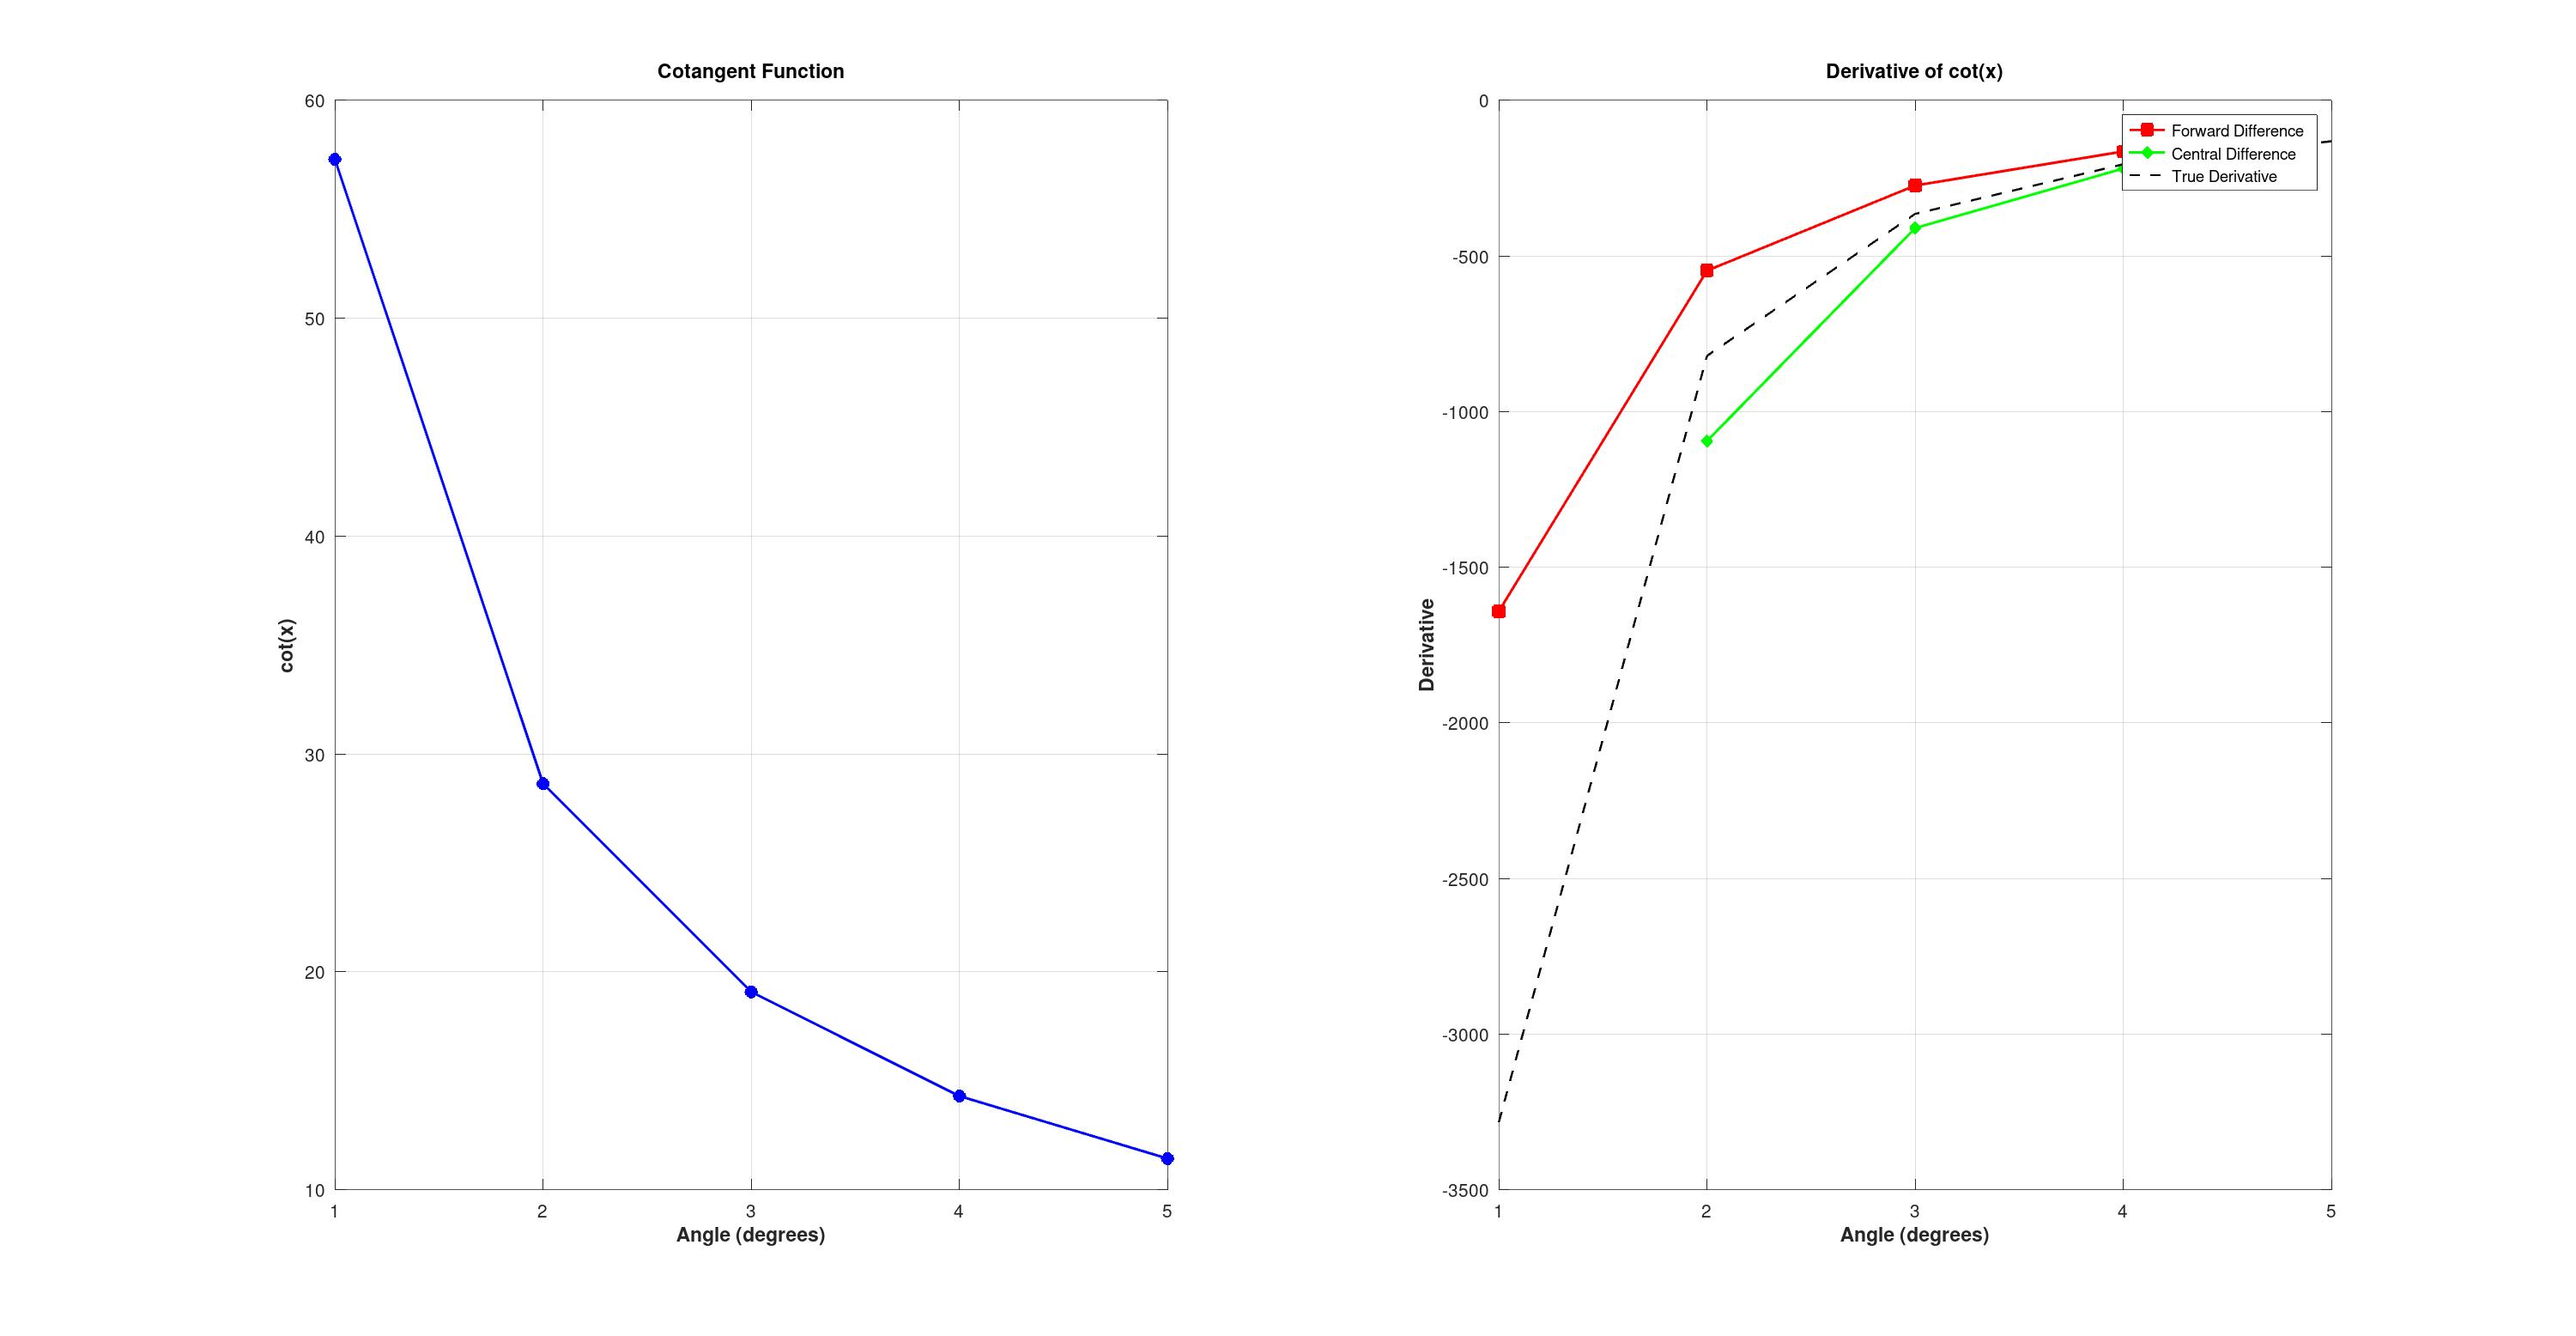
\includegraphics[width=0.9\textwidth]{a3.jpg}
  \caption{(Left) Cotangent function. (Right) Numerical derivatives using forward (red) and central (green) difference compared with the exact derivative (black dashed).}
\end{figure}

\section*{Conclusion}
Numerical differentiation using finite difference schemes successfully approximates the derivative of \(f(x) = \cot(x)\). Central difference is more accurate than forward difference due to its symmetric nature. The results validate that finite difference methods are effective for estimating derivatives of smooth functions when only discrete samples are available.
